\documentclass[12pt,a4paper]{article}

\usepackage[utf8]{inputenc}
\usepackage[T1]{fontenc}
\usepackage[french]{babel}

\usepackage{amsmath, amssymb}

\usepackage{graphicx}
\usepackage{caption}

\usepackage{siunitx} % Pour les unités

\usepackage{geometry}
\geometry{top=2cm, bottom=2.5cm, left=3cm, right=3cm}
\setlength{\parindent}{0pt}



\usepackage{enumitem}

\usepackage{hyperref}


\usepackage{tcolorbox}
\usepackage{xcolor}


\usepackage{paracol}
\usepackage{multicol}
\setlength{\columnseprule}{1pt}
\def\columnseprulecolor{\color{gray}}


\usepackage{import}
\usepackage{xifthen}
\usepackage{pdfpages}
\usepackage{transparent}
\usepackage{float}

\newcommand{\incfig}[1]{%
	\def\svgwidth{\columnwidth}
	\import{./figures/}{#1.pdf_tex}
}




\newcommand{\RomanNum}[1] %pour les chiffre romain
{\MakeUppercase{\romannumeral #1}}














\title{Projet structure en BA}
\author{}
\date{\today}

\begin{document}
	
	\counterwithin{section}{part}
	
	\maketitle
	
	\tableofcontents
	
	\newpage
	
	
	\part{Chapitre 1}
	
	\section{Présentation de l'ouvrage et description}
	
	\begin{itemize}
		\item Utilisation (habitaion, commercial, usine,...ect)
		\item Zone d'implantation et zone sismique.
		\item Géometrie du batiment et nombre d'étages (Hauteur totale, H d'étage, largeur, longeur, ...ect).
		\item Type de construction (construction mixte, en BA, en charpent, bois, ...ect).
		\item Type de structure (Structure mixte (voiles+poteaux), structure en autostable).
		\item Présentation du site d'installation.
	\end{itemize}
	
	
	\section{Caractéristique des matériaux}
	
	Les caractéristique du béton, de l'acier pour les armature ou pour la charpente ou bien du bois si la construction est en bois.
	
	\section{Prédimensionnement}
	
	\begin{tcolorbox}[colback=gray!20, colframe=black, title=Remarque]
		Le dimensionnement ce fait a l'ELS
	\end{tcolorbox}
	
	Les éléments prédimensionner sont : 
	
	\begin{itemize}
		\item Poteaux et poutres.
		\item Plancher \bigg( Dalles en corp creux (16+4 ou 20+5), dalles pleine \bigg).
		\item Voile.
		\item Balcon.
		\item Escalier.
	\end{itemize}
	
	\subsection{Poteaux}
	
	Le chargement du plancher se transmet a partir des poutrelles vers les poutres principale et puis finalment au poteaux.
	
	Et chaque poteau reprend la moitier des chargement des poutre comme montrer dans la figure 1.
	
	\vspace{\baselineskip}
	
	Les poutres principale sont celles dans les quelles repose les poutrelles (voir figure 1).
	
	\vspace{2cm}
		
	\begin{multicols}{2}
		
		
		\begin{figure}[H]
			\centering
			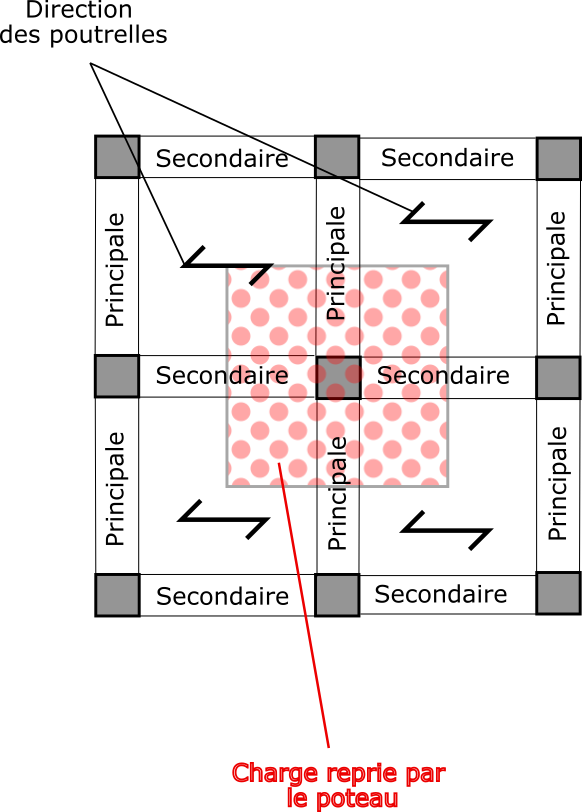
\includegraphics[width=1\linewidth]{figures/charge-sur-poteau}
			\caption{Charge que reprend le poteau}
			\label{fig:charge-sur-poteau}
		\end{figure}
		
		
		\columnbreak
		
		\begin{figure}[H]
			\centering
			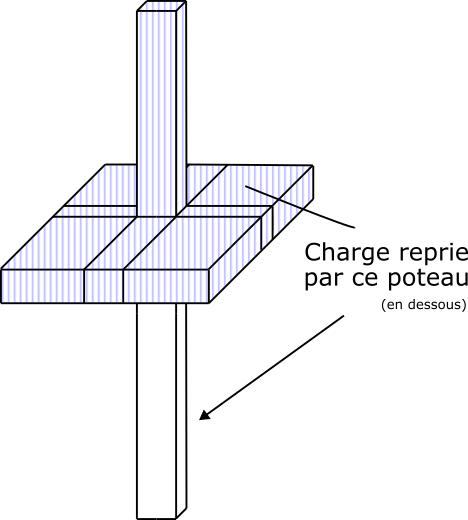
\includegraphics[width=1\linewidth]{figures/charge-reprie2}
			\caption{Charge que reprend le poteau (vue de face)}
			\label{fig:charge-reprie2}
		\end{figure}
		
		
	\end{multicols}
	
	
	\begin{tcolorbox}[colback=gray!20, colframe=black, title=Remarque]
		Le poids propre du poteau qui reprend les charge est prie en compte : 
		
		(Attention a pas calculer le poids d'un poteau deux fois lors du calcul de la descente de charge de l'étage inférieur)
		
		\begin{figure}[H]
			\centering
			\includegraphics[width=0.5\linewidth]{"figures/charge reprie 3"}
			\caption{Poids reprie totale}
			\label{fig:charge-reprie-3}
		\end{figure}
		
		
	\end{tcolorbox}
	
	
	\begin{tcolorbox}[colback=gray!20, colframe=black, title=Remarque]
		Lors du calcul des poids qui revient au poteau pour les poutres on prend en compte uniquement leur poids propre même si en réalité en dessus y'a aussi le revétement et l'enduit de platre par dessous mais ils sont négligable.
	\end{tcolorbox}
	
		
	\subsubsection{Calcul des chargements}
	
	Pour les poteaux, on aura le poids propre de chaque poutre qui est reprie, le poids du poteau dèn dessus si y'en a, et puis le plancher dont le poids est de :
	
	\paragraph{Plancher terrasse inaccessible} :
	
	\begin{figure}[H]
		\centering
		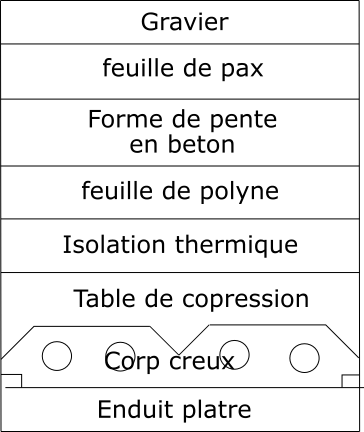
\includegraphics[width=0.4\linewidth]{figures/elements-plancher}
		\caption{Éléments d'un plancher terrase innaccesible}
		\label{fig:elements-plancher}
	\end{figure}
	
	
	\begin{itemize}
		\item Enduit platre = $0,2~\unit{kN\per m^{2}}$
		\item Hourdis + Dalle de copression = $2,8~\unit{kN\per m^{2}}$
		\item Isolation thermique = $0,16~\unit{kN\per m^{2}}$
		\item Feuille de polyne = $0,01~\unit{kN\per m^{2}}$
		\item Forme de pente en béton = $1,54~\unit{kN\per m^{2}}$
		\item Feuille de pax (étanchiéter multi couche) = $0,12~\unit{kN\per m^{2}}$
		\item Couche de gravier = $0,85~\unit{kN\per m^{2}}$
	\end{itemize}
	
	\[ g = 0,2+2,8+0,16+0,01+... = 5,68~\unit{kN\per m^{2}} \]
	
	
	\paragraph{Plancher courant} :
	
	Pour le placher courant on aura le sable pour revétement, l'isolation phonique et le carlage.
	
	\begin{itemize}
		\item Enduit = $0,4~\unit{kN\per m^{2}}$
		\item Hourdis + Dalle de copression = $2,8~\unit{kN\per m^{2}}$
		\item Cloison en brique = $0,9~\unit{kN\per m^{2}}$
		\item Isolation phonique = $0,1~\unit{kN\per m^{2}}$
		\item Couche de sable = $0,36~\unit{kN\per m^{2}}$
		\item Mortier de pose = $0,44~\unit{kN\per m^{2}}$
		\item Carrelage = $0,4~\unit{kN\per m^{2}}$
	\end{itemize}
	
	\[ g = 0,4 + 2,8 + 0,9 + 0,1 +... = 5,4~\unit{kN\per m^{2}} \]
	
	\paragraph{Surcharge d'exploitation} :
	
	\begin{itemize}
		\item Plancher terrasse : $Q = 1~\unit{kN\per m^{2}}$
		\item Plancher courant : $Q = 1,5~\unit{kN\per m^{2}}$
		\item Escalier : $Q = 2,5~\unit{kN\per m^{2}}$
		\item Balcon : $Q = 3,5~\unit{kN\per m^{2}}$
	\end{itemize}
	
	
	\begin{tcolorbox}[colback=gray!20, colframe=black, title=Remarque]
		Le poids des poutrelles sont considérer dans la table de copression (poids hourdis + T.copression = $2,8~\unit{kN\per m^{2}}$)
	\end{tcolorbox}
	
	
	
	
	
	
	\subsubsection{Dimensionnement}
	
	Pour trouver les dimension (a et b) du poteau a \underline{\textbf{l'ELS :}}
	
	\[ F = G + Q \qquad \text{ et } \quad S = a \cdot b \]
	
	\[ \sigma = \dfrac{F}{S} \quad \leq \quad \overline{\sigma}_{b} = \underset{ELS}{0,6 \cdot fc_{28}} \]
	
	\[ \Downarrow \]
	
	\[ a \cdot b \geq \dfrac{F}{\overline{\sigma}_{b}} \qquad \text{Avec F étant la charge qui revient au poteau} \]
	
	
	Selon le RPA : les dimension minimale des poteaux est en fonction des zones sismique :
	
	\begin{minipage}[t]{0.6\textwidth}
		\vspace{-2cm}
		\begin{equation}
			\begin{split}
				\min(a, b) &\geq 25~\unit{cm} \text{  en zones 	$\RomanNum{1}$ et $\RomanNum{2}$a } \\
				\min(a, b) &\geq 30~\unit{cm} \text{  en zones 	$\RomanNum{2}$b et $\RomanNum{3}$}
			\end{split}
			\label{dtr:RPA prédimensionnement poutre}
		\end{equation}
	\end{minipage}\hfill
	\begin{minipage}[b]{0.3\textwidth}
		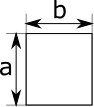
\includegraphics[width=0.5\linewidth]{figures/section-ab-rpa}
	\end{minipage}
	
	
	
	\begin{tcolorbox}[colback=gray!20, colframe=black, title=Remarque]
		Pour les poteau on peut diminuer la section pour les étage supérieur (chaque 3 étage???) contrairement au poutres, et le ferraillage se fait ainsi :
		
		\begin{figure}[H]
			\centering
			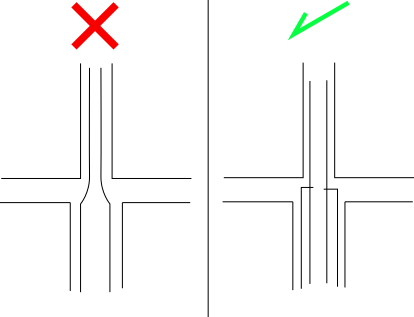
\includegraphics[width=0.7\linewidth]{figures/ferraillage-deux-poteau}
			\caption{ferraillage correct d'un poteau sans continuité}
			\label{fig:ferraillage-deux-poteau}
		\end{figure}
		
		
	\end{tcolorbox}
	
	
	
	
	\subsection{Dimensionnement du plancher}
	
	\[ H_{p} = \dfrac{L_{\max}}{22,5} \]
	
	Avec :
	
	$H_{p}$ : la hauteur du plancher.
	
	$L_{\max}$ : La plus grande travée (plus grande distance entre nue d'appuies).
	
	
	
	\[ \begin{cases}
		\text{si  } H_{p} < 16+4 = 20~\unit{cm} \text{  alors on choisie un plancher en 16+4} \\\\
		\text{sinon si  } 16+4 < H_{p} < 20+5 \text{  alors on va opter pour un plancher en 25 cm} 
	\end{cases} \]
	
	
	
	
	\subsection{Dimensionnement de la poutre}
	
	\subsubsection{Hauteur}
	
	\[ \dfrac{L_{\max}}{15} < h < \dfrac{L_{\max}}{10} \]
	
	
	\[ \text{Selon le RPA : } h \geq 30~\unit{cm} \]

	
	
	\subsubsection{Largeur}
	
	\[ 0,4 \cdot h \leq b \leq 0,7 \cdot h \]
	
	Avec $h$ étant la hauteur de la poutre.
	
	\[ \text{Selon le RPA : } b \geq 20~\unit{cm} \]
	
	
	\vspace{\baselineskip}
	
	\[ \text{Selon le RPA :} \quad \dfrac{h}{b} \leq 4 \]
	
	Ce réglement dit que la hauteur de la poutre dois étre inférieur a 4 fois ca largeur pour éviter un déversement.
	
	\[ b_{\max} \leq 1,5 \cdot h + b \]
	
	\vspace{\baselineskip}
	
	
	
	
	\begin{tcolorbox}[colback=gray!20, colframe=black, title=Remarque]
		Une poutre peut avoir de différent dimensions par rapport a une autre poutre par exemple une poutre principale avec une secondaire.
		
		\vspace{\baselineskip}
		
		Mais une même poutre ne peut avoir de différent section et doit assurer une continuité car un changement de section peut engdrer une concentration de contrainte de séisme sur la section réduite.
		
		\begin{figure}[H]
			\centering
			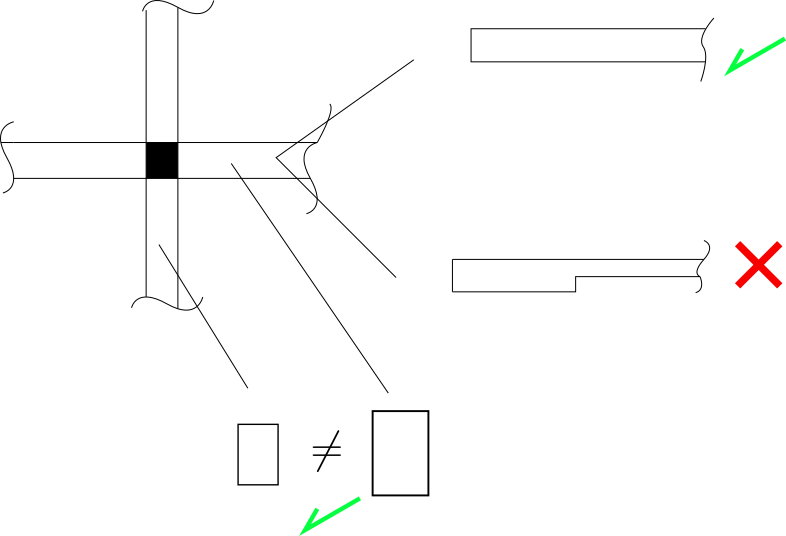
\includegraphics[width=0.7\linewidth]{figures/continuite-poutre}
			
			\vspace{1cm}
			
			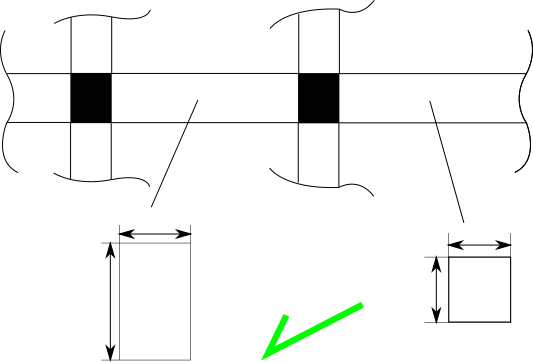
\includegraphics[width=0.5\linewidth]{figures/continuite-poutre2}
			\caption{Continuité des poutres}
			\label{fig:continuite-poutre}
		\end{figure}
		
		
	\end{tcolorbox}
	
	
	\begin{tcolorbox}[colback=gray!20, colframe=black, title=Remarque]
		On dimensionne la poutre dans une direction x avec $L_{x \:\max}$ de cette direction puis on dimensionne l'autre poutre (dans l'autre direction) avec le $L_{y \:\max}$ dans la direction y.
	\end{tcolorbox}
	
	
	\subsection{Dimensionnement du voile}
	
	\[ e = \dfrac{h_{e}}{20} \]
	
	Avec $h_{e}$ étant la hauteur d'étage moins la hauteur du plancher (c'est comme la distance entre nue d'appuie).
	
	Et selon le RPA : 
	
	\[ e_{min} = 15~\unit{cm} \]
	
	
	
	
	
	
	
	
	
	
	
	
	
	
	
	
	
	
	
	
	\part{Calculs des éléments}
	
	Le calcul des éléments se fera a l'ELU.
	
	
	\section{Calcul de l'acrotére}
	
	
	L'acrotére est un élements dans la terrasse, destiné à protéger les personnes 
	contre la chute et d’éviter le ruissellement d’eau sur la façade. Il est soumis uniqument a son poids propre avec une surcharge d'exploitation qui peut être l'échelle des pompiers, maintenance ou autre.
	
	
	
	\begin{figure}[H]
		\centering
		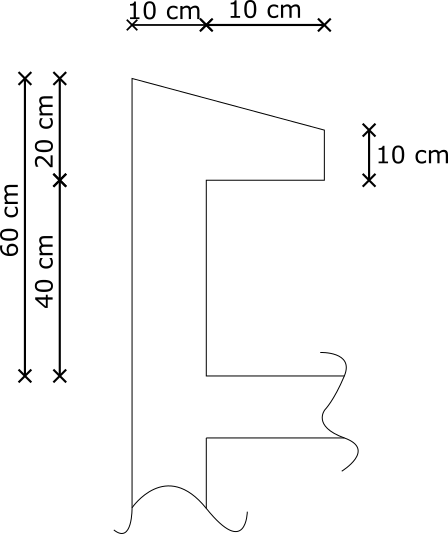
\includegraphics[width=0.4\linewidth]{figures/chapitre-2/dim-acrotere}
		\caption{Forme et dimension de l'acrotére}
		\label{fig:dim-acrotere}
	\end{figure}
	
	
	
	\vspace{\baselineskip}
	
	\subsection{Charges}
	
	
	L'acrotére est soumis a la flexion composée.
	
	\begin{figure}[H]
		\centering
		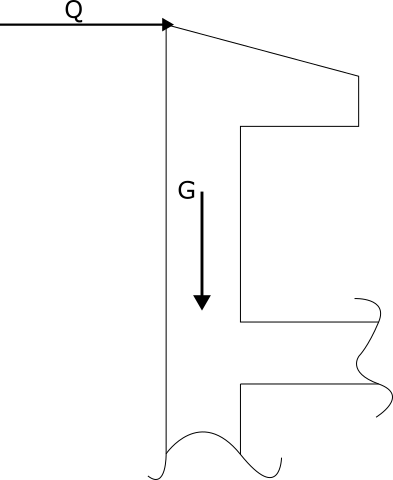
\includegraphics[width=0.3\linewidth]{figures/chapitre-2/charge-acrotere}
		\caption{Chargement appliquer a l'acrotére}
		\label{fig:charge-acrotere}
	\end{figure}
	
	
	Le calcul se fait pour 1m linéaire.
	
	
	
	\[ G = V \cdot \rho_{ba} = \left( 40 \cdot 10 + 20 \cdot 10 + \dfrac{20 \cdot 10}{2} \right) \cdot 25  = 1,75 ~\unit{kN} \text{ Pour 1m linéaire} \]
	
	
	Et depuis le DTR charge et surcharge d'exploitation on a $q = 1 ~\unit{kN\per m}$
	
	\[ Q = q \cdot 1 ~\unit{ml} = 1 ~\unit{kN} \]
	
	
	\subsection{Diagramme des efforts}
	
	Sous flexion composée
	
	\begin{figure}[H]
		\centering
		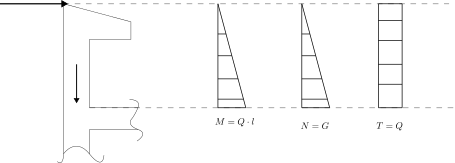
\includegraphics[width=0.7\linewidth]{figures/chapitre-2/efforts-acrotere}
		\caption{Effort interne de l'acrotére}
		\label{fig:efforts-acrotere}
	\end{figure}
	
	
	
	
	\begin{tcolorbox}[colback=gray!20, colframe=black, title=Remarque]
		L'effort normale est triangulaire car plus on descend plus on a le volume qui augmente.
	\end{tcolorbox}
	
	
	\vspace{\baselineskip}
	
	
	
	\section{Calcul des poutrelles}
	
	
	Les poutrelles reprenne la moitié de l'hourdis a droite et la moitié a gauche.
	
	
	\begin{figure}[H]
		\centering
		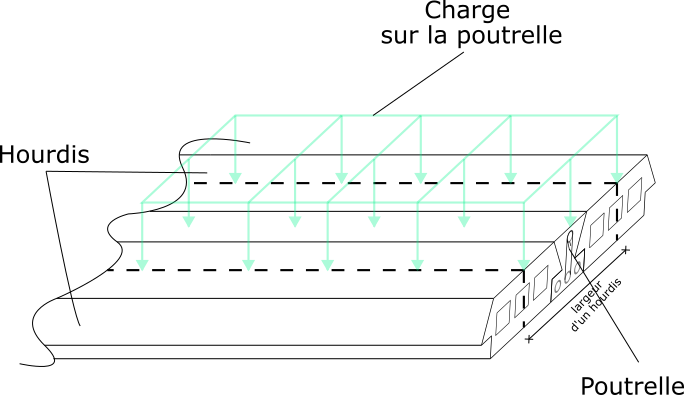
\includegraphics[width=0.7\linewidth]{figures/chapitre-2/charge-poutrelle}
		\caption{Charges reprie par une poutrelle.}
		\label{fig:charge-poutrelle}
	\end{figure}
	
	
	
	On dimensionnne uniquement celle qui est la défavorable (celle qui reprend le plus de charges).
	
	\begin{tcolorbox}[colback=gray!20, colframe=black, title=Remarque]
		Les poutrelles sont continue sur toute la longeur, cad la poutrelle a un chapeau (ferraillge) qui assure la continuité. 
	\end{tcolorbox}
	
	\vspace{\baselineskip}
	
	\subsection{Les charges}
	
	
	
	Comme on calcul uniqument la poutrelle la plus chargé donc :
	
	
	\[ 
	\begin{array}{l c l}
		\text{Plancher courant} &\quad& \text{Plancher terrasse} \\
		g = 5,4 ~\unit{kN\per m^{2}} &\quad& g = 5,68 ~\unit{kN\per m^{2}} \\
		q = 1,5 ~\unit{kN\per m^{2}} &\quad& q = 1 ~\unit{kN\per m^{2}}
	\end{array}
	 \]
	
	Le plus sollicité c'est le plancher courant avec :
	
	\[ Q = 1,35 \cdot g + 1,5 \cdot q = 1,35 \cdot 5,4 + 1,5^{2} = 9,54 ~\unit{kN\per m^{2}} \]
	
	
	
	\subsection{Calcul des efforts}
	
	On différente méthode de calcul :
	
	\begin{itemize}
		\item Méthode des trois moments.
		\item Méthode de Caquot.
		\item Méthode forfaitaire.
	\end{itemize}
	
	
	\subsubsection{Méthode forfaitaire}
	
	
	
	\paragraph{Conditions et méthode de calcul}:
	
	
	\begin{itemize}
	
		\item Les charges d'exploitations doivent être modérée
	
		\[ Q \leq 500 ~\unit{kg\per m^{2}} \]
		
		\[ Q \leq 2 \cdot G \]
		
		
		\item Fissuration est peu nuisible (fissuration peu préjudiciable).
		
		\item Le rapport entre deux travée successive est de :
		
		\[ 0,8 \leq \dfrac{L_{i + 1}}{L_{i}} \leq 1,25 \]
		
		\item Les poutrelles doivent être semi-encastrée
		
		\begin{tcolorbox}[colback=gray!20, colframe=black, title=Remarque]
			
			Un encastrement parfait c'est quand : inertie du poteau >>> inertie de la poutre.
			
			\vspace{\baselineskip}
			
			Semi-encastrée $I_{poteau} \approx I_{poutre}$
			
			\vspace{\baselineskip}
			
			Le moment en appuie de rive varie selon l'encastrement.
			 
		\end{tcolorbox}
	
	\end{itemize}
	
	\vspace{3\baselineskip}
	
	
	On suppose que les moments sont isostatique, puis on multiplie par des coefficient pour trouvée les moments de rives et hyperstatiques.
	
	\begin{figure}[H]
		\centering
		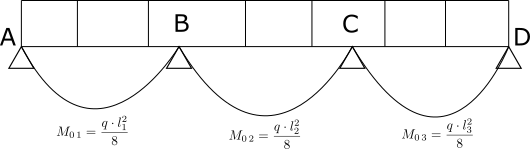
\includegraphics[width=0.7\linewidth]{figures/chapitre-2/forfaitaire-statique}
		\caption{Les moments statiques}
		\label{fig:forfaitaire-statique}
	\end{figure}
	
	
	\paragraph{Moments au appuie de rive}:
	
	
	\[ M_{A} = 0,15 \cdot M_{0\,1} \]
	
	\[ M_{D} = 0,15 \cdot M_{0\,3} \]
	
	
	\paragraph{Moments au appuie intermidiaire}:
	
	\[
	\begin{cases}
		0,6 \cdot M_{0} \quad\text{ Pour une poutre a 2 travée} \\
		0,5 \cdot M_{0} \quad\text{ Pour les appuie voisin d'appuie de rive} \\
		0,4 \cdot M_{0} \quad\text{ Pour les autres appuie intermidiare a plus de 3 travée.}
	\end{cases}
	\]	
	
	\paragraph{Moments en travée}:
	
	\[
	\begin{cases}
		M_{t} \geq \dfrac{1 + 0,3 \cdot \alpha}{2} \cdot M_{0} \quad\text{ Travée intermidiare.} \\ \\
		M_{t} \geq \dfrac{1,2 + 0,3 \cdot \alpha}{2} \cdot M_{0} \quad\text{ Travée de rive.}
	\end{cases}
	\]	
	
	Avec \[ \alpha = \dfrac{Q}{G + Q} \]
	
	\paragraph{Vérification}:
	
	Pour chaque travée il faut vérifier que :
	
	\[ M_{t\,i} + \dfrac{M_{w} + M_{e}}{2} \geq \max 
	\begin{cases}
		(1 + 0,3 \cdot \alpha) \cdot M_{0\,i} \\
		1,05 \cdot M_{0\,i}
	\end{cases}
	 \]
	
	\vspace{3\baselineskip}
	
	\begin{tcolorbox}[colback=gray!20, colframe=black, title=Remarque]
		On peut aussi trouvée les moments graphiquement on superposant le moment isostatique a partir des moments en appuie.
	\end{tcolorbox}
	
	
	
	
	
	
	
	
	
	
	\section{Calcul des escaliers}
	
	On fait le calcul a l'ELU et des vérification a l'ELS.
	
	\vspace{\baselineskip}
	
	
	Les escalier sont en béton armé (Dalle pleinne)
	
	Coposée de palier et de la paillase, sur cette derniére on a a les marches et contre-marches.
	
	\vspace{\baselineskip}
	
	On a deux types de palier : le palier de départ et le palier intermediare.
	
	\vspace{\baselineskip}
	
	L'escalier se repose sur les poutres ou bien les poutres paliéres, ou bien aussi sur les longrines pour les RDCs.
	
	
	
	\begin{figure}[H]
		\centering
		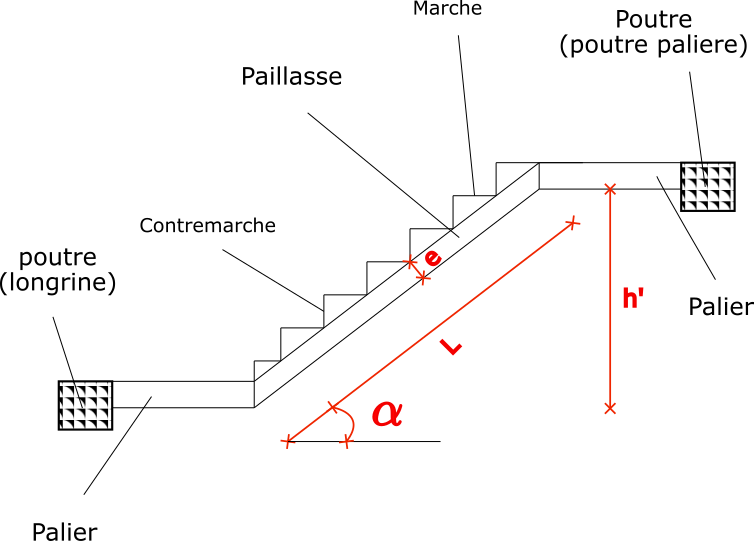
\includegraphics[width=0.7\linewidth]{figures/chapitre-2/escalier}
		\caption{}
		\label{fig:escalier}
	\end{figure}
	
	
	
	
	\subsection{Les charges sur l'escalier}
	
	\subsubsection{Palier}
	
	Poids propre + Revêtements + garde corps + charge d'exploitation.
	
	\subsubsection{Paillasse}
	
	Poids propre + Revêtements + garde corps + poids des marches et des contre marches + charge d'exploitation.
	
	
	
	\subsection{Modéles d'escalier}
	
	
	\begin{figure}[H]
		\centering
		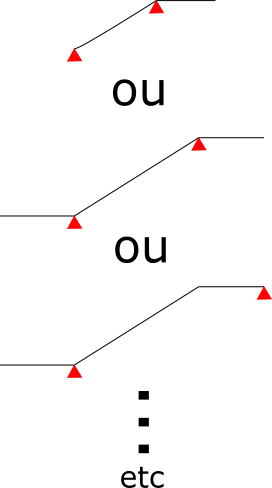
\includegraphics[width=0.3\linewidth]{figures/chapitre-2/modele-escalier}
		\caption{}
		\label{fig:modele-escalier}
	\end{figure}
	
	
	\subsection{Projection}
	
	On projete la longeur L de la paillasse
	
	
	\begin{figure}[H]
		\centering
		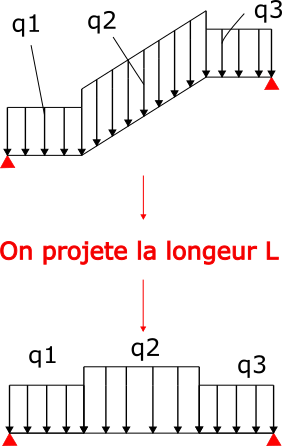
\includegraphics[width=0.3\linewidth]{figures/chapitre-2/modele-escalier2}
		\caption{}
		\label{fig:modele-escalier2}
	\end{figure}
	
	
	
	
	
	\subsection{Dimensionement des marches et des contremarches}
	
	On utilise la formule de Blondel qui est empirique :
	
	\[ 2 \cdot h + g = 60 \sim 64 ~\unit{cm} \]
	
	
	Avec :
	
	$h$ : la hauteur de la marche (la contremarche).
	
	$g$ : giron, profondeur de la marche (la marche, partie sur laquelle on pose le pied.)	
	
	
	
	\subsection{Dimensionement de la paillasse}
	
	\[ \dfrac{L_{0}}{30} \leq e \leq \dfrac{L_{0}}{20} \]
	
	avec $L_{0}$ longeur entre deux appuie non projetée. 
	
	
	
	
	
	
	
	
	
	
	
	
	
	
	
	
	
	
	
	
	
	
	
	
	
	
	
	
	
	
	
	
	
	
	
	
	
	
\end{document}